\chapter{}{{Solar Forecasting Using Numerical Weather Prediction Models}}{Solar Irradiance Forecasting Using Numerical Weather Prediction Models}

\subchapter{Overview}
For a days-ahead forecast horizon, utilizing Numerical Weather Prediction (NWP) models, which predict the evolution of the atmospheric system have been shown to be more useful \cite{thesis_zach}. The NWP models derive their initial conditions from different ground and airborne sensors from across the world. Based on thermodynamic equations describing the physical processes occurring in atmosphere, they forecast different weather variables into the forecast horizon. The National Oceanic and Atmospheric Administration (NOAA) operates a variety of NWP models with their spatial resolution ranging from approximately 10 km - 50 km, and their temporal resolution typically being 1 hour or 3 hours \cite{multimodel_bestpractices}. 

\par Solar forecasting researchers have successfully employed meteorological forecasts from NWP models for forecasting applications for years. The making of a weather forecast involves assessing the current weather situation, assimilating observational information, and projecting this initial state into the future based on the laws of thermodynamics. Weather forecasting employs a set of equations that describe the flow of fluids, being run over a geographic area. Several parameterizations of physical processes are carried out, based on the physical and statistical representations of the physical process. This is useful to approximate the bulk effects of the physical processes.

\par One of the major challenges faced in this process is determining the range of area to observe. The further the forecasting of the weather conditions, i.e, higher the forecast horizon, wider is the range of area that needs to be observed. Multiple weather prediction models, both global and regional, depending on the spatial domain, are maintained by the National Oceanic and Atmospheric Administration (NOAA). Global Forecast System (GFS) is one of the widely-known global weather prediction models, which represents the atmospheric state as a superposition \restoregeometry\noindent of wave functions. It covers the entire globe at a base horizontal resolution of $28km$ between grid points, predicting weather out to $16$ days. Within continental United States, North American Mesoscale (NAM), Rapid Refresh (RAP), High Resolution Rapid Refresh (HRRR) are the popular regional weather prediction models, each having it's own advantages. The NAM Forecast System follows a complex cloud prediction scheme accounting for the internal cloud processes, and thus has better cloud parameterizations over RAP and HRRR. 

\par In this work, we developed machine learning models to forecast solar irradiance on multiple dual-axis tracking (array A), fixed-axis (array B) and single-axis tracking (array E) solar arrays. The irradiance predictions were made 24 hours into the future, at a one-hour temporal resolution. The NAM Forecast System, which can predict parameters describing cloudiness \cite{multimodel_nam}, was input to these predictive models. A weather forecast dataset spanning NAM data for the years 2017 and 2018 was created, though a few forecasts are missing sporadically. 

\par In order to gauge the effect of different weather variables specified by the NAM Forecast System on the solar irradiance predictions, the following were evaluated: air temperature, geopotential height, cloud cover, visibility, wind speed, dew point temperature, air pressure, downward shortwave radiation flux, downward longwave radiation flux, and humidity. Using \textit{random forests}, the more relevant of these weather variables were identified. It was observed that the irradiance readings from the solar farm for each of the arrays were influenced more by the surface temperature, downward short-wave radiation flux, total cloud cover, and atmospheric height. Thus, the remaining weather variables were discarded. This enabled a cut in computational cost of modeling and also led to an improvement in the performance of the models.

\par Each of the weather variables in the NAM Forecast System are projected 36 hours into the future, at a 1-hour temporal resolution. Of these, the effect of the first 24 feature projections on the target solar irradiance was analyzed based on the \textit{mutual information} statistical measure. It was found that the weather variable for a particular target hour offset in the forecast horizon depends on only 6 feature projections following the target hour offset, and 6 feature projections preceding the target hour offset. Separate machine learning models were trained, and the efficacy of the proposed input-selection scheme was tested. 

\par The performance of this input-selection scheme was compared with the methodology followed by Jones \cite{thesis_zach}. It was observed that the input-selection scheme resulted in an average improvement in mean absolute error ($MAE$) across machine learning models by 19.05\%, 19.68\% and 10.65\% for the dual-axis tracking, fixed-axis and single-axis solar arrays respectively. \textit{Random forests} achieved a best performance for such predictive models, with an $MAE$ of 72.63 $W/m^2$, 44.94 $W/m^2$ and 63.60 $W/m^2$ for each of the arrays.

\par The effect of the geographic expansion of weather forecast coverage was analyzed by including the $3$ x $3$ and $5$ x $5$ \textit{geo shapes}, wherein weather forecasts data from eight and twenty four NAM data grid cells centered around the NAM data grid representing Athens, Georgia were incorporated respectively. Such a spatial expansion was assessed for the attribute-selected weather forecast data, obtained by incorporating the input-selection scheme. It was found that the geographic expansion had a detrimental effect on the performance of the machine learning models, and had a marginal improvement with respect to the $1$ x $1$ \textit{geo shape} only for random forests, with the $5$ x $5$ \textit{geo shape} resulting in $MAE$ of 69.38 $W/m^2$, 43.62 $W/m^2$, 61.99 $W/m^2$ for the dual-axis tracking, fixed-axis and single-axis tracking solar arrays respectively.

\subchapter{North American Mesoscale (NAM) Weather Prediction Model}
\par The North American Mesoscale (NAM) Forecast System is based on the Weather Research and Forecasting (WRF) model infrastructure, following non-hydrostatic dynamics and thus enabling vertical momentum estimations. It provides high resolution forecasts over North America for a forecast horizon of 84 hours, the first 36 of which are at a one hour temporal resolution, and the remaining thereafter, at a 3 hour temporal resolution. The forecasts are published for a grid spanning approximately $12km$ x $12 km$ across the continental United States, which are released four times daily at 00h, 06h, 12h and 18h UTC.

\begin{figure}[ht]
    \begin{center}
    	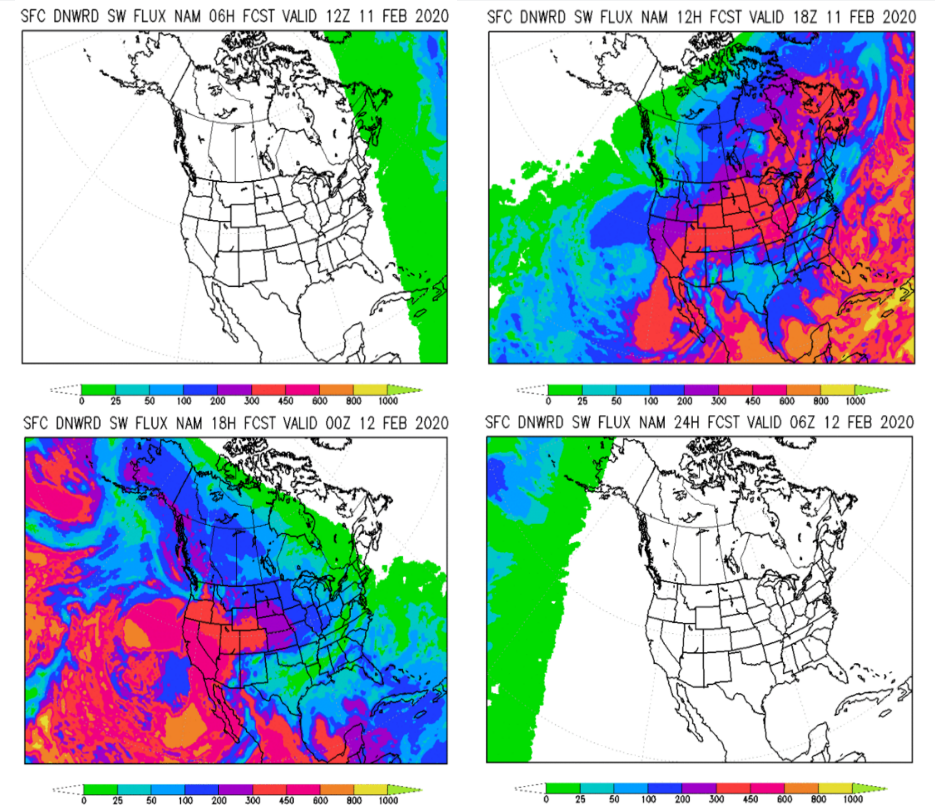
\includegraphics[width=0.85\textwidth]{chapter3/fig_nam_dswrf.png}
    	\caption[Downward shortwave radiation flux parameter for 06h, 12h, 18h, 24h UTC forecasts in a day for NAM Forecast System]{Downward Shortwave Radiation Flux parameter from NAM data over North America domain for 06h forecast (top-left), 12h forecast (top-right), 18h forecast (bottom-left) and 24h forecast (bottom-right) UTC for 11th February, 2020.}
    	\label{fig:fig_nam_dswrf}
    \end{center}
\end{figure}

\par In general, the NWP models cannot realize the  physical phenomenon occurring within an individual grid. Vertical redistribution of heat and moisture can easily occur between mesoscale grids resulting in sub grid-scale variations in convection. The NAM Forecast System repeatedly nudge the temperature and moisture profiles in a grid towards decreasing the convective instability. Moreover, the wider forecast horizon of the NAM Forecast System requires it to model the radiative properties within the clouds effectively \cite{multimodel_rtm}. The NAM models handle this by implementing columnar Radiative Transfer Models (RTMs), which parameterize the cloud properties for every vertical level individually.

\par Dozens of weather variables are available in a NAM model data grid pertaining to environmental components such as altitude, atmospheric pressure, atmospheric radiation, air temperature, water vapour, atmospheric winds, precipitation, soil properties and cloud cover. Each of these are spread across 60 vertical levels in a 0 - 3 km layer, and across 39 pressure levels from 50mb to 1000mb at 25mb intervals. From among these variables, in Fig.~\ref{fig:fig_nam_dswrf}\footnote{NAM forecast snapshots retrieved from: \url{https://www.emc.ncep.noaa.gov/mmb/mmbpll/etapll}}, the averaged \textit{downward short-wave radiation flux} over North America for the four forecasts on 11th February, 2020 is reported.

\subsubchapter{Data Collection}
\subsubsection*{Weather Forecasts}
\par As mentioned in 3.1.1, North American Mesoscale (NAM) Forecast System data was collected from the years 2017 and 2018 for experiments. From this data, surface-level variables as described in Table \ref{Tab:table_nam_variables} were retrieved and analyzed. NAM Forecast System projects different weather parameters 84 hours into the future. The first 36 feature projections in the forecast horizon are at a 1-hour temporal resolution, and subsequent 48 hours of the forecast horizon has feature projections at a 3-hour temporal resolution. In this work, we consider the first 24 feature projections (which are at a 1-hour temporal resolution) for each of the weather variables along with their corresponding target pyranometer readings. 

\begin{table}[h]
\begin{center}
    \caption{NWP-NAM weather variables used in model development}
    \label{Tab:table_nam_variables}
    \begin{tabular}{ c c c}
    	\toprule
    	\textbf{Label} & \textbf{Description} & \textbf{Unit} \\
    	\midrule
    	PRES\_SFC & Air Pressure & $Pa$\\
    	HGT\_SFC & Geopotential Height & $gpm$ \\
    	HGT\_TOA & Height at Planetary Boundary Layer & $gpm$ \\
    	TMP\_SFC & Air Temperature & $K$\\
    	VIS\_SFC & Visibility & $m$\\
    	UGRD\_TOA & U-Component of Wind Speed & $m/s$\\
    	VGRD\_TOA & V-Component of Wind Speed & $m/s$\\
    	DSWRF\_SFC & Downward Short-Wave Radiation Flux & $W/m^2$\\
    	DLWRF\_SFC & Downward Long-Wave Radiation Flux & $W/m^2$\\
    	TCC\_EATM & Total Cloud Cover & $\%$ \\
    	\bottomrule
    \end{tabular}
\end{center}
\end{table}

\subsubsection*{Temporal Features}
\par In this work, temporal features were designed so as to include the \textit{time of day} and \textit{time of year} representations of the forecasts, which incorporate the periodicity in time\footnote{In \cite{thesis_zach}, Jones attempted to use the \textit{time of day} and \textit{time of year} representations by scaling the epoch representing the reference time (in nanoseconds) with the inverse of $8.64e+13$ (number of nanoseconds in a day) and $3.1536e+16$ (number of nanoseconds in a year) respectively, and including their \textit{sine} and \textit{cosine values}. However, these do not appear to be correct as they do not capture the periodicity of the reference time.}. The \textit{time of day} was computed by scaling the number of seconds in the reference time with the inverse of $8.64e+4$ (number of seconds in a day); and the \textit{time of year} was computed by scaling the day of the year with the inverse of $365$ or $366$, depending on whether it is a leap year or not. The sine and cosine values of these measures were added as the temporal features. Such \textit{time of day} representations make the temporal features pertaining to the target hour in the forecast horizon different from that of the reference time. Thus, temporal features representing the target hours in the forecast horizon were also included along with their corresponding predictors.

\subsubsection*{Irradiance Observations}
\par The target irradiance observations are obtained from three solar arrays in the solar farm, namely array A, array B and array E, representing a dual-axis tracking array, fixed axis array with 200$^{\circ}$(SW) azimuth, and a single-axis tracking array respectively. Each of the solar arrays are installed with thermopile pyranometers from different manufacturers such as Kipp \& Zonen\footnote{\url{https://www.kippzonen.com/}}, and LICOR\footnote{\url{https://www.licor.com/}}. The thermopile pyranometers have a black absorptive surface which uniformly absorbs the solar radiation across the short-wave solar spectrum, i.e, between 0.2 $\mu m$ and 3 $\mu m$. 

\begin{figure}[ht]
    \begin{center}
    	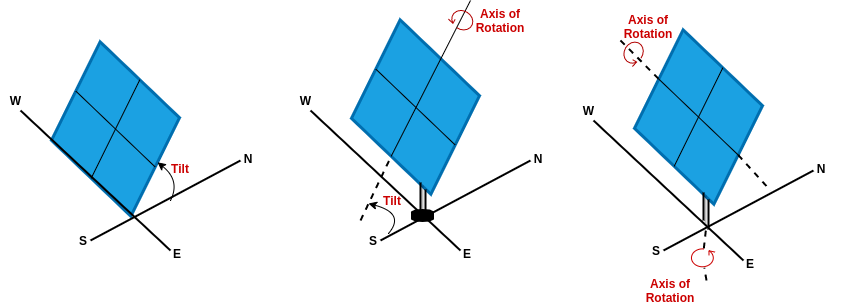
\includegraphics[width=0.85\textwidth]{chapter3/fig_pyranometers.png}
    	\caption[Fixed axis, Single-axis tracking, Dual-axis tracking Solar Arrays]{Fixed axis (left), Single-axis tracking (center), Dual-axis tracking (right) Solar Arrays.}
    	\label{fig:fig_pyranometers}
    \end{center}
\end{figure}

The fixed axis solar array has limited exposure to the sun, owing to the change in position of the sun during the day from morning to night. Thus, the solar radiation captured by this solar array is reduced. Though this limitation is minimized by installing the fixed solar array at an optimized tilt angle, the solar radiation captured by solar tracking arrays is still considerably higher. In order to maximize the overall solar energy captured, it is necessary to ensure that the angle of incidence of the sunlight on the solar array is constantly perpendicular. This is achieved with the help of single-axis trackers (horizontal and vertical), which have one degree of freedom acting as an axis of rotation; and dual-axis trackers which have two degrees of freedom acting as axes of rotation normal to one another \cite{irradiance_solartracker}. This ability to move along the axes enhances the morning and afternoon performance of the solar tracking systems.

\par While the irradiance observations from the solar arrays are received every five seconds, the NWP NAM model data is available only for four reference times in a day, i.e 00h, 06h, 12h, 18h UTC through 2017 and 2018. Thus, for the target hours in the forecast horizon of all the reference times in 2017 and 2018, for which the NWP NAM model data was collected, the irradiance observations were sampled. In Fig.~\ref{fig:fig_average_irradiance}, the average monthly solar radiation captured by the dual-axis tracking, fixed-axis and single-axis tracking solar arrays through 2017 is shown. It can be observed that the solar radiation captured by the tracking arrays (dual-axis and single-axis) is consistently higher than that captured by the fixed axis array.

\begin{figure}[ht]
    \begin{center}
    	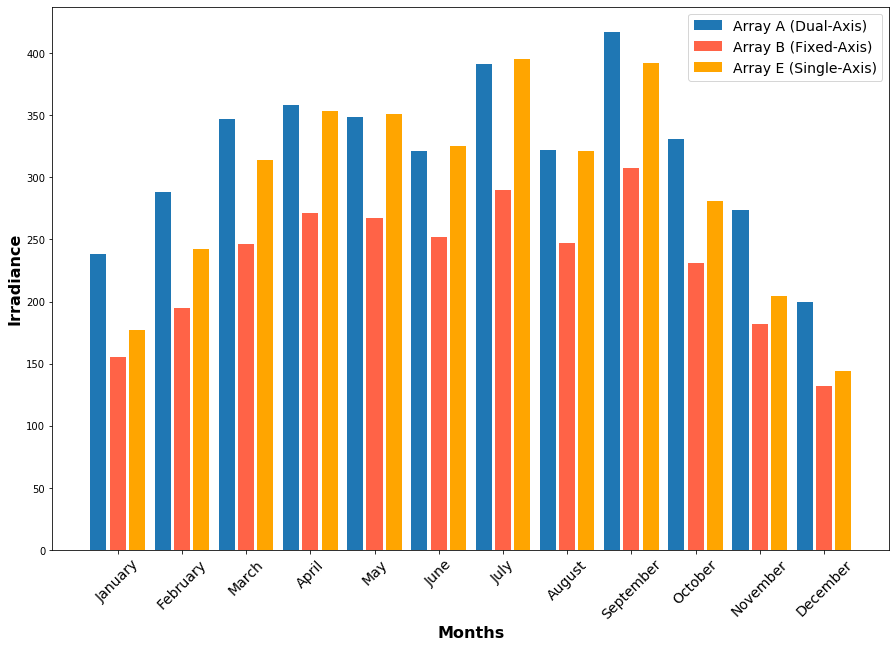
\includegraphics[width=0.85\textwidth]{chapter3/fig_average_irradiance.png}
    	\caption[Average monthly solar radiation captured by dual-axis tracking, fixed-axis and single-axis tracking solar arrays through 2017.]{Average monthly solar radiation captured by dual-axis tracking, fixed-axis and single-axis tracking solar arrays through 2017.}
    	\label{fig:fig_average_irradiance}
    \end{center}
\end{figure}

\subsubchapter{Evaluating Impact of Weather Variables on Irradiance Observations}
\par Mutual information is the measure between two possibly multi-dimensional variables, which quantifies the amount of information obtained from one variable about the other. The relationship detected between the variables can involve either mean, variance or even the higher moments \cite{feature_selection_mi}. The most straightforward and widespread approach towards estimating mutual information follows partitioning the supports of $X$ and $Y$ into bins of finite size, and approximating the sum in the following way:
\begin{equation}\label{eq:eq_mi}
I(X, Y) \approx I_{binned}(X, Y) \equiv \sum_{ij} p(i, j) . log(\frac{p(i, j)}{p_x(i).p_y(j)})
\end{equation}

\par In this work, the mutual information measure was estimated using the \textit{scikit-learn}\footnote{\url{https://scikit-learn.org/stable/}} machine learning software, which makes use of a non-parametric method based on entropy estimation from the \textit{k-nearest neighbors} as described in \cite{feature_selection_mi} and \cite{feature_selection_mi2}. Mutual information measure was calculated for different weather variables from the NAM data and corresponding irradiance observations from the solar arrays as described in the previous subsections. From among the weather variables, it was observed that downward shortwave radiation flux, air temperature, height at planetary boundary layer and total cloud cover have a mutual information score greater than 0.1, indicating a relatively higher dependency on the irradiance observations.

\par Downward shortwave radiation flux is the total amount of shortwave radiation that reaches the earth's surface, and is a major component of the total solar radiation on the surface of the earth. Thus, it is the most direct parameter in the estimation solar irradiance, and the high mutual information score between this weather variable and the irradiance observations from the solar farm is understandable. By absorbing the incoming solar radiation, the Earth warms up, and its temperature rises. As long as the amount of incoming radiative flux is greater than the outgoing radiative flux, the Earth will continue to warm. Thus, the air temperature at the surface is essential in estimating the amount of heat absorbed at that particular location, which in turn reveals information about the amount of solar radiation absorbed by the thermopiles in the pyranometers. 

\par The influence of clouds on solar irradiance is significant. In the absence of visible clouds, aerosols, precipitable water and other atmospheric conditions affect the transmission of solar radiation through atmosphere. In cloudy conditions though, the clouds absorb a significant amount of the shortwave radiation, making variables like total cloud cover, which is the fraction of the sky covered by visible clouds essential. The planetary boundary layer (PBL) is the lowest part of the atmosphere which is directly influenced by its contact with the planetary surface. The structure of turbulence within this layer is mainly governed by the PBL height, which is higher during the day, and lower and more stable during nighttime \cite{feature_selection_pbl1}. PBL height characterizes the planetary boundary layer in a fairly integrated manner and affects the weather parameters such as cloud cover and heat flux \cite{feature_selection_pbl2}. This makes PBL height an important parameter in predicting solar irradiance.

\par For the machine learning models to be able to capture and reconstruct the underlying relationship between input-output data pairs effectively, input selection is essential. By removing the redundant and misleading data, input selection often helps in reducing the computational costs, and improves the accuracy. Several approaches have been defined in literature for the purpose of input selection. In addition to assessing the mutual information scores, we used \textit{random forests} to identify the more important weather variables, as they provide an in-built feature selection.

\par Random forests employ tree-based strategies, which naturally rank inputs based on how well they improve the purity of the node. They are an ensemble learning technique constructed over a variety of randomized decision trees, each of which is built over a random extraction of features and data observations. The training of these randomized decision trees is done with the objective of decreasing the \textit{Gini Impurity}, and the features which help in decreasing this measure are selected \cite{feature_selection_rf}. Thus, random forests help determine the importance of the features in this manner. It was observed that the weather parameters with higher mutual information scores also received high feature importance scores through this technique, thus validating the dependence of the target irradiance observations on this set of parameters.

\par In \cite{thesis_zach}, Jones used 37 weather attributes, of which one corresponds to the weather data at the reference time and 36 are feature projections at an one-hour temporal resolution in the forecast horizon, as the predictor variables for machine learning models. In this work, a forecast horizon of 24 hours was selected, and the relationship between the weather attributes in this forecast horizon and the irradiance observations corresponding to the target hours in this forecast horizon was studied. 

\begin{figure}[htb]
    \begin{center}
    	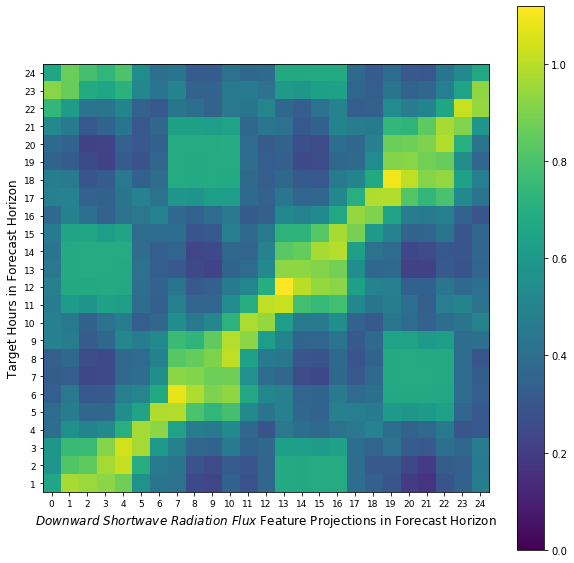
\includegraphics[width=0.65\textwidth]{chapter3/fig_mi_forecast_target.png}
    	\caption[Mutual information between Downward Shortwave Radiation Flux feature projections in forecast horizon and irradiance observations for corresponding target hours from fixed-axis solar array]{Mutual information between feature projections of Downward Shortwave Radiation Flux in the forecast horizon and irradiance observations for corresponding target hours along fixed-axis solar array.}
    	\label{fig:fig_mi_forecast_target}
    \end{center}
\end{figure}

\par As was noted earlier, downward shortwave radiation flux was the most important NAM weather variable with respect to the irradiance observations in the solar farm. In Fig.~\ref{fig:fig_mi_forecast_target}, the mutual information between the feature projections of this weather variable and the corresponding irradiance observations from fixed-axis solar array are represented in a heatmap, wherein, different colours in the colour-bar depict the amount of mutual information measure. It can be observed that the irradiance observations from fixed axis array for a particular target hour are relatively more dependent on only a certain number of feature projections in the forecast horizon. Thus, for the machine learning models trained for each target hour in the forecast horizon, feature projections from six hours ahead, and six hours prior were considered as predictors. 
\par For the first six target hours in the forecast horizon which do not necessarily have six prior feature projections, desired number of feature projections were selected from the end. Similarly, for the last six target hours in the forecast horizon which do not necessarily have six subsequent feature projections, desired number of feature projections were selected from the beginning of the forecast horizon. Such a feature projection selection is justified because it is more likely for the same reference time in two consecutive days to have similar weather conditions. Thus, following this input selections scheme, the NAM model data contributes 13 feature projections for each of the four environmental attributes described earlier, eight temporal features (four for the reference time of the forecast, four for the target hour offset from the reference time) towards the post-processing of solar irradiance from each of the solar arrays using machine learning models.

\subchapter{Experiment Setup}
\par In this chapter, two series of experiments are performed towards predicting solar irradiance on the dual-axis tracking, fixed-axis and single-axis tracking solar arrays. In the first series of experiments, solar irradiance forecasting using Numerical Weather Prediction (NWP) models such as North American Mesoscale (NAM) Forecast System is investigated, replicating the modeling methodology employed by Jones in \cite{thesis_zach}. This is compared with the processed NAM dataset obtained by incorporating the input selection scheme described in 3.2.2. 

\par In this work, 24-hour \textit{persistence models} were used to set a baseline for the more sophisticated machine learning models. Based on the assumption that conditions remain unchanged between the current time and a future time, 24-hour \textit{persistence models} measure the solar irradiance at a particular time $t$ based on the irradiance measured at $t-24$. Making use of such a trivial model as baseline provides a reference for improving the machine learning models. 

\par Several machine learning algorithms such as \textit{Least-Squares Linear Regression} (LSLR), \textit{k-Nearest Neighbors} (KNN), \textit{Support Vector Regression} (SVR), \textit{Decision Trees} (DT), \textit{Random Forests} (RF) and \textit{Extreme Gradient Boosted Trees} (XGBT) were used for the purpose of forecasting. Python-based machine learning softwares \textit{scikit-learn} and \textit{xgboost}\footnote{\url{https://github.com/dmlc/xgboost}} were used for the implementations of these machine learning algorithms. Randomized cross-validated grid search was employed to identify the optimal set of hyperparameters, ranges for each of which were selected around the default values set for them in the \textit{scikit-learn} implementations.

\par Weather variables from the NAM Forecast System were used as predictors for the machine learning models, and the irradiance observations from the solar arrays were used as target variables. Each of the weather variables are projected 36 hours into the future at a one-hour temporal resolution. As a part of the input-selection scheme, select feature projections were picked from the important weather variables, depending on the target hour in the forecast horizon. Prediction of target irradiance was done for a day-ahead forecast horizon, i.e, solar irradiance was predicted 24 hours into the future at a one hour temporal resolution. Models were trained on data collected during 2017, and evaluated against data collected during 2018. In the first series of experiments, the performance of the models, with and without employing the input-selection scheme was compared.

\par Jones \cite{thesis_zach} reported evaluation metrics such as \textit{mean absolute error} ($MAE$) and \textit{coefficient of determination} ($R^2$). $MAE$ is a more natural and unambiguous measure of average error, and is extremely useful in evaluating average-model performance. An evaluation metric such as $R^2$ helps in providing a reference point for comparing the model results with results from other literature. Owing to these advantages, in this work, both the evaluation metrics were retained to facilitate a consistent comparison. In addition, the correlation coefficient ($r$) is reported as well.

\par Model results were analyzed in two schemes: mean of the evaluations for each forecast hour in the forecast horizon ($Overall$); mean of the evaluations for sets of six forecast hours in the forecast horizon, i.e, $1 - 6$, $7 - 12$, $13 - 18$ and $19 - 24$. $MAE$ was estimated for each of these forecast horizon segments by taking an average of the metric across each of the target hours in the segment. However, for $R^2$ and $r$, this was performed by flattening the predictions and ground-truth values for multiple target hours in the forecast horizon segment into single lists, and computing the metrics over these lists. Such an analysis helped in realizing the performance of the models specifically for different periods in the day. 

\par Geographic expansion of forecast coverage by including additional weather forecasts specific to areas surrounding the target location is considered to improve the solar irradiance forecasting capabilities. In the second series of experiments, the effect of such a spatial expansion is investigated, by including the feature projections of weather variables from a grid of cells around the NAM data grid representing Athens, as predictors to the machine learning models. A geographic expansion from the $1$ x $1$ grid to other \textit{geo shapes} such as $3$ x $3$ and $5$ x $5$ is investigated for the \textit{K-Nearest Neighbors}, \textit{Random Forests} and \textit{Extreme Gradient Boosted Trees} algorithms. Each of these methodologies are further explained in finer detail.

\subsubchapter{Irradiance Forecasting with NAM Forecast System}
\par For the replication study, North American Mesoscale (NAM) weather forecast data and target irradiance data from the solar farm at the University of Georgia were collected for the years 2017 and 2018. For a forecast horizon of 24 hours, planar surface features from the NAM Forecast System such as air pressure, geopotential height, height at planetary boundary layer, air temperature, u-component of wind speed, v-component of wind speed, downward short-wave radiation flux and downward long-wave radiation flux were used. 

\par As mentioned in 3.2.2, it was determined that weather variables such as air temperature, total cloud cover, atmospheric height and downward short-wave radiation flux from among the surface-level planar features affected the solar irradiance predictions more. Hence, the other weather variables were omitted. Depending on the target hour offset in the forecast horizon, select feature projections were picked for the weather variables, so as to be included in the NAM dataset. This was done by selecting 13 from among the 37 weather attributes at a one-hour temporal resolution such that, six followed the reference time of the target hour offset, six preceded the reference time of the target hour offset, and one corresponded to the reference time of the target hour offset. In order to choose an ideal set of parameters for the machine learning models, \textit{hyperparameter tuning} was performed with the help of a randomized cross-validated grid search. 

\par The weather forecast data obtained by both methodologies was input to several machine learning models, which were trained on data collected during 2017, and evaluated against data collected during 2018. The results obtained by both methodologies, i.e with and without incorporating the input selection scheme, were compared and analyzed.

\vspace{0.5cm}

\subsubchapter{Geographic Expansion of Forecast Coverage}
\par Lorenz et al. \cite{expansion_lorenz} found that expanding the forecast region to approximately $100 km$ x $100 km$ resulted in an improvement in day-ahead solar forecasting. They performed a spatial averaging across the region, by taking  an arithmetic mean of the weather variables from the surrounding weather data grid cells. In contrast, Sanders et. al. \cite{publication_sanders} and Jones \cite{thesis_zach} performed a distance-dependent weighted averaging, by including the weather variables from the surrounding weather data grid cells as predictors to the machine learning models.

\begin{figure}[ht]
    \begin{center}
    	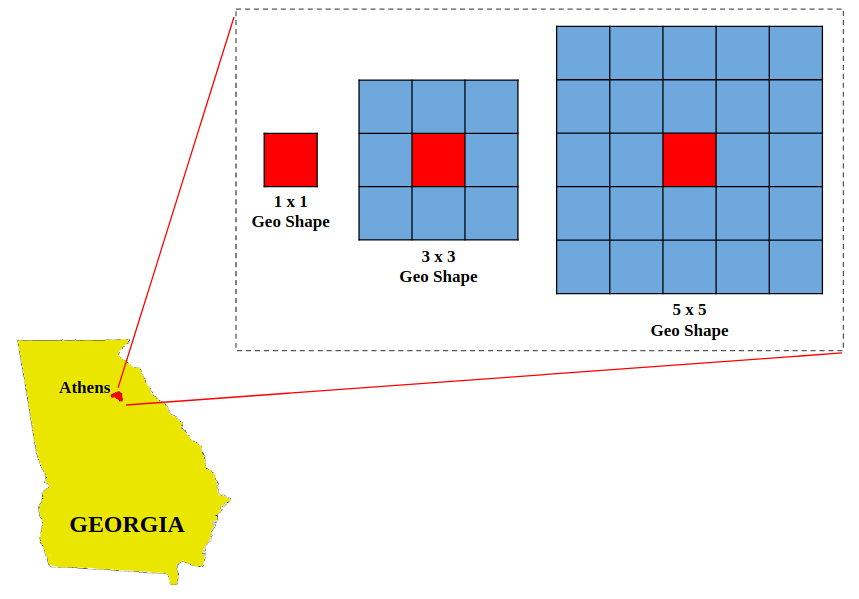
\includegraphics[scale=0.23]{chapter3/fig_geoshapes.png}
    	\caption[Geographic expansion of forecast coverage around Athens NAM model data grid]{Geographic expansion of forecast coverage with 1 x 1 Geo Shape representing Athens NAM model data grid, 3 x 3 Geo Shape and 5 x 5 Geo Shape representing grid of cells around Athens.}
    	\label{fig:fig_geoshapes}
    \end{center}
\end{figure}

\par Jones \cite{thesis_zach} trained \textit{k-nearest neighbors} and \textit{random forest} algorithms for $3$ x $3$, $5$ x $5$ and $7$ x $7$ \textit{geo shapes}, each reflecting a spatial expansion up to $36km$ x $36km$, $60km$ x $60km$ and $84km$ x $84km$ respectively. As shown in Figure~\ref{fig:fig_geoshapes}, each of the \textit{geo shapes} represent eight, fifteen and forty eight NAM weather forecast data grid cells centered around Athens, Georgia. They realized that including the weather forecasts from the surrounding data grid cells resulted in an improved day-ahead solar forecasting, though it was observed that the improvement diminished as the \textit{geo shape} grew larger. Additionally, Jones \cite{thesis_zach} also noted that the $3$ x $3$ \textit{geo shape}, equivalent to a $36km$ x $36km$ area was optimal. 

\par In this work both the schemes were compared: one in which GHI from the surrounding grids is averaged, and other in which weather variables from surrounding cells are included as predictors. It was observed that the latter helped in improving the performance of the models more. Thus, a geographic expansion of weather forecast coverage was carried out with $3$ x $3$ and $5$ x $5$ \textit{geo shapes}, resulting in a spatial expansion upto $60km$ x $60km$. The dataset set up using the input selection scheme described in 3.2.2, was used to determine the effect of geographic expansion.

\vspace{0.3cm}
\subchapter{Results and Discussion}
\subsubsection*{Assessment of Model Performance with and without Input Selection Scheme}
\par In this work, an input selection scheme as described in 3.2.2 was incorporated towards selecting features for the machine learning models. The performance of the machine learning models using both the methodologies, i.e. with and without the input selection scheme were compared for dual-axis tracking solar array, fixed-axis solar array and single-axis tracking solar array. As a part of this scheme, the key differences between Jones' dataset and the one used in this work, towards training with the machine learning models are as follows:
\begin{itemize}
    \itemsep0em
    \item Jones \cite{thesis_zach} hadn't considered the \textit{total cloud cover} weather variable in the NAM weather dataset
    \item from among the other surface-level NAM weather variables used, only air temperature, height at planetary boundary layer and downward shortwave radiation flux were considered
    \item instead of the 37 weather attributes for each of the weather variables, select feature projections depending on the target hour offset were chosen as predictor variables
    \item $1$ x $1$ \textit{geo shape} was selected instead of $3$ x $3$ (which Jones \cite{thesis_zach} had found to be optimal)
    \item \textit{time of day} and \textit{time of year} encodings were modified to incorporate periodicity of the reference time in a particular day or in a particular year
\end{itemize}

%\par Based on these differences, the two NAM datasets were used as input to different machine learning models. Separate machine learning models were trained for each of the target hour offsets between 1 and 24, and their 

\begin{table}[h]
\begin{center}
        \caption[Comparing performance of machine learning algorithms trained against dual-axis tracking array using NAM Forecast System data, with and without input selection.]{Comparing performance of machine learning algorithms trained against dual-axis tracking array utilizing NAM Forecast System data: (a) without input selection (upper), (b) with input selection (lower)}
%    \vspace{0.2cm}
    \label{Tab:fs_array_a}
    \begin{tabular}{@{}p{5.3em}ccccccccc@{}}
    \toprule
    & \textbf{Metric} & \textbf{Horizon} & \textbf{PER} & \textbf{LSLR} & \textbf{SVR} & \textbf{KNN} & \textbf{DT} & \textbf{RF} & \textbf{XGBT} \\ \cmidrule(l){1-10} 
    \multirow{10}{5em}{Without Input Selection} & \multirow{5}{*}{$MAE$} & $1 - 6$ & 153.32 & 231.00 & 88.38 & 98.73 & 98.34 & 74.38 & 73.03 \\
                                              &                   & $7 - 12$ & 153.91 & 231.06 & 89.83 & 101.77 & 105.17 & 77.14 & 76.97 \\
                                              &                   & $13 - 18$ & 154.16 & 232.15 & 89.08 & 106.56 & 98.31 & 74.43 & 75.64 \\
                                              &                   & $19 - 24$ & 161.43 & 243.04 & 89.88 & 104.15 & 98.19 & 75.02 & 76.69 \\
                                              &                   & $Overall$ & 155.71 & 234.31 & 89.29 & 102.80 & 100.00 & \textbf{75.24} & 75.58 \\ \cmidrule(lr){2-10}
                                              & \multirow{5}{*}{$R^2$} & $1 - 6$ & 0.46 & 0.31 & 0.85 & 0.78 & 0.71 & 0.86 & 0.86 \\
                                              &                   & $7 - 12$ & 0.45 & 0.29 & 0.84 & 0.78 & 0.68 & 0.85 & 0.84 \\
                                              &                   & $13 - 18$ & 0.45 & 0.31 & 0.84 & 0.77 & 0.71 & 0.86 & 0.85 \\
                                              &                   & $19 - 24$ & 0.41 & 0.25 & 0.84 & 0.77 & 0.71 & 0.85 & 0.85 \\
                                              &                   & $Overall$ & 0.44 & 0.29 & 0.84 & 0.77 & 0.70 & 0.85 & 0.85 \\ 
    \midrule
    \multirow{3}{5em}{Relative Imp. in $MAE$ (\%)} & & & & & & & & & \\
    & & $Overall$ & --- & 52.17 & 17.76 & 28.97 & 10.91 & 3.47 & 1.02 \\ 
    & & & & & & & & & \\
    \midrule
    \multirow{10}{5em}{Input Selection}
                                              & \multirow{5}{*}{$MAE$} & $1 - 6$ & 153.32 & 107.08 & 70.63 & 68.54 & 85.74 & 70.21 & 71.65 \\
                                              &                   & $6 - 12$ & 153.91 & 114.52 & 73.82 & 72.35 & 90.57 & 72.92 & 74.6 \\
                                              &                   & $13 - 18$ & 154.16 & 115.03 & 73.34 & 73.12 & 87.65 & 72.6 & 75.77 \\
                                              &                   & $19 - 24$ & 161.43 & 111.68 & 75.93 & 78.04 & 92.39 & 74.78 & 77.23 \\
                                              &                   & $Overall$ & 155.71 & 112.08 & 73.43 & 73.02 & 89.09 & \textbf{72.63} & 74.81 \\ \cmidrule(lr){2-10}
                                              & \multirow{5}{*}{$R^2$} & $1 - 6$ & 0.46 & 0.84 & 0.88 & 0.88 & 0.78 & 0.88 & 0.87 \\
                                              &                   & $7 - 12$ & 0.45 & 0.83 & 0.86 & 0.86 & 0.76 & 0.87 & 0.86 \\
                                              &                   & $13 - 18$ & 0.45 & 0.82 & 0.86 & 0.86 & 0.77 & 0.87 & 0.86 \\
                                              &                   & $19 - 24$ & 0.41 & 0.82 & 0.85 & 0.85 & 0.74 & 0.86 & 0.85 \\
                                              &                   & $Overall$ & 0.44 & 0.83 & 0.86 & 0.86 & 0.76 & 0.87 & 0.86 \\ 
    \bottomrule
    \end{tabular}
\end{center}
\end{table}

\par For the dual-axis tracking solar array, all the machine learning models performed exceedingly well with respect to the baseline 24-hour \textit{persistence} models, which was expected. A substantial improvement was observed for all the machine learning models built using weather forecast data without incorporating the input-selection scheme. In particular, using the input selection scheme helped in improving the $MAE$ of simple \textit{linear regression} by 52.17\%. There was a considerable improvement in the performance of \textit{support vector regression} and \textit{k-nearest neighbors} algorithms as well, with the $MAE$ reducing by 17.76\% and 28.97\% respectively. Each of these algorithms is greatly affected by a higher dimensionality and quality of data, and by weeding out weather variables and their feature projections which have a lesser influence on the target irradiance, the improvement in performance of these models can be justified.   

\par Ensemble tree-based methods have the intrinsic ability to calculate feature importance, and account for the possible correlations between the variables. Thus in general, they perform better than the linear regression methods. For the dual-axis tracking array, random forests had the best performance with an $MAE$ of 72.63 $W/m^2$, and extreme gradient boosted trees recorded an overall $MAE$ of 74.81 $W/m^2$. The improvement over the performance of the same algorithms without incorporating the input selection scheme was 3.47\% and 1.02\% respectively.

\par While the random forests performed the best, considerable improvements in performance as a result of incorporating the input selection scheme were seen in the \textit{support vector regression} and \textit{k-nearest neighbors} algorithms. Overall, there was an average improvement in $MAE$ by 19.05\% across the machine learning models, with \textit{random forests} having the best $MAE$ with 72.63 $W/m^2$ for the dual-axis tracking solar array.

\begin{table}[h]
\begin{center}
    \caption[Comparing performance of machine learning algorithms trained against fixed-axis solar array using NAM Forecast System data, with and without input selection.]{Comparing performance of machine learning algorithms trained against fixed-axis solar array utilizing NAM Forecast System data: (a) without input selection (upper), (b) with input selection (lower)}
%    \vspace{0.2cm}
    \label{Tab:fs_array_b}
    \begin{tabular}{@{}p{5.3em}ccccccccc@{}}
    \toprule
    & \textbf{Metric} & \textbf{Horizon} & \textbf{PER} & \textbf{LSLR} & \textbf{SVR} & \textbf{KNN} & \textbf{DT} & \textbf{RF} & \textbf{XGBT} \\ \cmidrule(l){1-10} 
    \multirow{10}{5em}{Without Input Selection} & \multirow{5}{*}{$MAE$} & $1 - 6$ & 111.23 & 151.79 & 55.018 & 61.10 & 62.81 & 47.09 & 47.21 \\
                                              &                   & $7 - 12$ & 111.51 & 147.12 & 56.65 & 63.78 & 62.05 & 48.32 & 49.56 \\
                                              &                   & $13 - 18$ & 111.97 & 151.09 & 55.64 & 68.70 & 64.64 & 48.19 & 49.22 \\
                                              &                   & $19 - 24$ & 117.15 & 159.29 & 56.11 & 66.53 & 62.28 & 47.65 & 49.44 \\
                                              &                   & $Overall$ & 112.96 & 152.32 & 55.85 & 65.03 & 62.95 & \textbf{47.81} & 48.86 \\ \cmidrule(lr){2-10}
                                              & \multirow{5}{*}{$R^2$} & $1 - 6$ & 0.59 & 0.54 & 0.89 & 0.85 & 0.80 & 0.90 & 0.89 \\
                                              &                   & $7 - 12$ & 0.58 & 0.55 & 0.89 & 0.85 & 0.80 & 0.89 & 0.88 \\
                                              &                   & $13 - 18$ & 0.58 & 0.55 & 0.89 & 0.83 & 0.78 & 0.89 & 0.88 \\
                                              &                   & $19 - 24$ & 0.55 & 0.50 & 0.89 & 0.83 & 0.80 & 0.89 & 0.88 \\
                                              &                   & $Overall$ & 0.58 & 0.54 & 0.89 & 0.84 & 0.80 & 0.89 & 0.88 \\ 
    \midrule
    \multirow{3}{5em}{Relative Imp. in $MAE$ (\%)} & & & & & & & & & \\
    & & $Overall$ & --- & 51.92 & 16.47 & 28.42 & 10.90 & 6.00 & 4.36 \\ 
    & & & & & & & & & \\ 
    \midrule
    \multirow{10}{5em}{Input Selection}
                                              & \multirow{5}{*}{$MAE$} & $1 - 6$ & 111.23 & 69.81 & 44.26 & 42.77 & 55.30 & 42.94 & 44.66 \\
                                              &                   & $6 - 12$ & 111.51 & 74.74 & 47.19 & 46.72 & 55.96 & 45.16 & 46.77 \\
                                              &                   & $13 - 18$ & 111.97 & 79.63 & 47.02 & 47.02 & 56.65 & 45.14 & 46.79 \\
                                              &                   & $19 - 24$ & 117.15 & 68.75 & 48.13 & 49.67 & 56.48 & 46.51 & 48.69 \\
                                              &                   & $Overall$ & 112.96 & 73.24 & 46.65 & 46.55 & 56.09 & \textbf{44.94} & 46.73 \\ \cmidrule(lr){2-10}
                                              & \multirow{5}{*}{$R^2$} & $1 - 6$ & 0.59 & 0.89 & 0.91 & 0.92 & 0.84 & 0.92 & 0.91 \\
                                              &                   & $7 - 12$ & 0.58 & 0.88 & 0.90 & 0.90 & 0.84 & 0.91 & 0.90 \\
                                              &                   & $13 - 18$ & 0.58 & 0.87 & 0.90 & 0.90 & 0.83 & 0.91 & 0.90 \\
                                              &                   & $19 - 24$ & 0.55 & 0.88 & 0.89 & 0.89 & 0.83 & 0.90 & 0.89 \\
                                              &                   & $Overall$ & 0.58 & 0.88 & 0.90 & 0.90 & 0.84 & 0.91 & 0.90 \\ 
    \bottomrule
    \end{tabular}
\end{center}
\end{table}


\par In general, it's expected that the performance of the models degrades as the forecast horizon increases. However, Jones \cite{thesis_zach} did not observe such a pattern, with sometimes, even the $7 - 12$ hour forecast horizon performing worse than $13 - 18$ and $19 - 24$ hours forecast horizons. Such a trend though, was realized in the results obtained by incorporating the input selection scheme. By and large, most of the models displayed a trend where the error increased (performance degraded) with the target hour in the forecast horizon. Considering the overall improvement in performance, it can be inferred that this indicates an improvement in the short-term forecasting ability of the models.

\par Similar trends were also observed in the performance of the machine learning models for irradiance predictions on the fixed-axis solar array (in Table~\ref{Tab:fs_array_b}). The \textit{random forests} performed the best with an $MAE$ of 44.94 $W/m^2$. This model achieved an improvement of 6\% due to the incorporation of the input-selection scheme. In contrast, \textit{random forests}, which were also the best-performing model without incorporating the input-selection methodology (as followed by Jones \cite{thesis_zach}), achieved a $MAE$ of 47.81 $W/m^2$. In all, the input-selection scheme achieved an average improvement of 19.68\% in $MAE$ across all the machine learning models.

\vspace{1em}

\begin{table}[h]
\begin{center}
    \caption[Comparing performance of machine learning algorithms trained against single-axis tracking array using NAM Forecast System data, with and without input selection.]{Comparing performance of machine learning algorithms trained against single-axis tracking solar array utilizing NAM Forecast System data: (a) without input selection (upper), (b) with input selection (lower)}
    \label{Tab:fs_array_e}
%    \vspace{0.2cm}
    \begin{tabular}{@{}p{5.3em}ccccccccc@{}}
    \toprule
    & \textbf{Metric} & \textbf{Horizon} & \textbf{PER} & \textbf{LSLR} & \textbf{SVR} & \textbf{KNN} & \textbf{DT} & \textbf{RF} & \textbf{XGBT} \\ \cmidrule(l){1-10} 
    \multirow{10}{5em}{Without Input Selection} & \multirow{5}{*}{$MAE$} & $1 - 6$ & 128.64 & 174.61 & 67.52 & 83.58 & 77.53 & 56.81 & 57.67 \\
                                              &                   & $7 - 12$ & 128.97 & 176.21 & 70.13 & 86.63 & 82.25 & 60.32 & 61.40 \\
                                              &                   & $13 - 18$ & 129.25 & 176.39 & 68.79 & 91.08 & 81.01 & 58.54 & 60.15 \\
                                              &                   & $19 - 24$ & 135.35 & 182.16 & 68.70 & 87.62 & 82.42 & 58.42 & 60.85 \\
                                              &                   & $Overall$ & 130.55 & 177.34 & 68.79 & 87.23 & 80.80 & \textbf{58.52} & 60.02 \\ \cmidrule(lr){2-10}
                                              & \multirow{5}{*}{$R^2$} & $1 - 6$ & 0.53 & 0.48 & 0.88 & 0.79 & 0.77 & 0.89 & 0.88 \\
                                              &                   & $7 - 12$ & 0.53 & 0.46 & 0.87 & 0.79 & 0.75 & 0.75 & 0.87 \\
                                              &                   & $13 - 18$ & 0.53 & 0.48 & 0.87 & 0.77 & 0.75 & 0.88 & 0.87 \\
                                              &                   & $19 - 24$ & 0.49 & 0.45 & 0.87 & 0.78 & 0.74 & 0.88 & 0.87 \\
                                              &                   & $Overall$ & 0.52 & 0.47 & 0.87 & 0.78 & 0.75 & 0.88 & 0.87 \\ 
    \midrule
    \multirow{3}{5em}{Relative Imp. in $MAE$ (\%)} & & & & & & & & & \\
    & & $Overall$ & --- & 48.39 & 5.9 & 24.65 & 2.08 & -8.68 & -8.46 \\ 
    & & & & & & & & & \\ 
    \midrule
    \multirow{10}{5em}{Input Selection}
                                              & \multirow{5}{*}{$MAE$} & $1 - 6$ & 128.64 & 87.52 & 62.29 & 61.71 & 75.62 & 61.37 & 62.93 \\
                                              &                   & $6 - 12$ & 128.97 & 95.30 & 65.77 & 65.98 & 81.80 & 64.09 & 65.55 \\
                                              &                   & $13 - 18$ & 129.25 & 93.47 & 64.29 & 65.75 & 76.77 & 63.50 & 65.73 \\
                                              &                   & $19 - 24$ & 135.35 & 89.84 & 66.57 & 69.47 & 82.28 & 65.44 & 66.18 \\
                                              &                   & $Overall$ & 130.55 & 91.53 & 64.73 & 65.73 & 79.12 & \textbf{63.60} & 65.10 \\ \cmidrule(lr){2-10}
                                              & \multirow{5}{*}{$R^2$} & $1 - 6$ & 0.53 & 0.86 & 0.88 & 0.88 & 0.80 & 0.89 & 0.88 \\
                                              &                   & $7 - 12$ & 0.53 & 0.85 & 0.87 & 0.86 & 0.77 & 0.87 & 0.87 \\
                                              &                   & $13 - 18$ & 0.53 & 0.85 & 0.87 & 0.86 & 0.79 & 0.88 & 0.87 \\
                                              &                   & $19 - 24$ & 0.49 & 0.85 & 0.86 & 0.86 & 0.77 & 0.87 & 0.87 \\
                                              &                   & $Overall$ & 0.52 & 0.85 & 0.87 & 0.86 & 0.78 & 0.88 & 0.87 \\ 
    \bottomrule
    \end{tabular}
\end{center}
\end{table}

\par In the present investigation of incorporating the input-selection scheme, the most interesting results were seen with the single-axis tracking solar array predictions (in Table~\ref{Tab:fs_array_e}). For the \textit{k-nearest neighbors} algorithm, trends followed the predictions for the other solar arrays reported so far, with a reduction in $MAE$ by 24.65\%. For the predictions with \textit{support vector regression}, a reduction in $MAE$ by 5.9\% was observed. However, this relative improvement in performance was less in magnitude as compared to those observed for dual-axis tracking array predictions and fixed-axis array predictions. In addition, using the tree-based ensemble methods such as \textit{random forests} and \textit{extreme gradient boosted trees}, a degradation in performance was recorded, with the $MAE$ increasing by 8.68\% and 8.46\%. Though \textit{random forests} still performed the best with an $MAE$ of 63.6 $W/m^2$, this performance paled in comparison to that of the \textit{random forests} without incorporating the input-selection scheme, where an $MAE$ of 58.52 $W/m^2$ was obtained. To explain this, the corresponding data and code were investigated. No errors in data processing were found. Moreover, a systematic error would have affected all the arrays, which wasn't the case. 


\subsubsection*{Evaluating Effect of Geographic Expansion of Forecast Coverage}
\par Better performing algorithms in 3.3.1 such as \textit{k-nearest neighbors}, \textit{random forests} and \textit{extreme gradient boosted trees} were retrained on dual-axis tracking, fixed-axis and single-axis tracking solar arrays and corresponding weather forecast data for the year 2017, and evaluated against data belonging to the year 2018. The performance of these models for each of the \textit{geo shapes} $1$ x $1$, $3$ x $3$ and $5$ x $5$ was compared and analyzed.

\par Using the \textit{k-nearest neighbors} algorithm to predict the day-ahead solar irradiance on dual-axis tracking solar array, it was observed that the geographic expansion had a slightly detrimental effect on the performance. Expanding to $3$ x $3$ \textit{geo shape} resulted in increasing the $MAE$ by 1.59\%, and increasing the weather forecast coverage to $5$ x $5$ \textit{geo shape} resulted in increasing the $MAE$ by 0.44\%. For these models, the $1$ x $1$ performed best with a $MAE$ of 73.01 $W/m^2$.

\begin{table}[h]
\begin{center}
    \caption{Evaluating effect of geographic expansion of forecast coverage for dual-axis tracking array.}
    \begin{tabular}{c c c c c c c c c c c}
        \toprule
        \multirow{2}{*}{\textbf{Metric}} & \multirow{2}{*}{\textbf{Horizon}} & \multicolumn{3}{c}{\textbf{KNN}} & \multicolumn{3}{c}{\textbf{RF}} & \multicolumn{3}{c}{\textbf{XGBT}}\\
        \cmidrule{3-11}
         &  & 1x1 & 3x3 & 5x5 & 1x1 & 3x3 & 5x5 & 1x1 & 3x3 & 5x5 \\
        \midrule
        \multirow{5}{*}{$MAE$} & $1 - 6$ & 68.61 & 69.68 & 69.02 & 68.53 & 67.90 & 66.69 & 71.04 & 69.23 & 85.32 \\
        & $7 - 12$ & 72.52 & 73.72 & 72.77 & 72.40 & 71.40 & 69.38 & 73.51 & 72.44 & 87.16 \\
        & $13 - 18$ & 72.86 & 74.27 & 73.06 & 70.82 & 69.85 & 68.39 & 73.69 & 71.91 & 87.47 \\
        & $19 - 24$ & 78.05 & 78.99 & 78.47 & 74.99 & 74.46 & 73.06 & 77.92 & 76.02 & 90.02 \\
        & $Overall$ & \textbf{73.01} & 74.17 & 73.33 & 71.68 & 70.90 & \textbf{69.38} & 74.04 & \textbf{72.40} & 87.49 \\
        \midrule
        \multirow{5}{*}{$R^2$} & $1 - 6$ & 0.88 & 0.87 & 0.87 & 0.88 & 0.88 & 0.89 & 0.87 & 0.88 & 0.84 \\
        & $7 - 12$ & 0.86 & 0.85 & 0.86 & 0.87 & 0.87 & 0.88 & 0.86 & 0.86 & 0.84 \\
        & $13 - 18$ & 0.86 & 0.85 & 0.85 & 0.87 & 0.87 & 0.88 & 0.86 & 0.87 & 0.83 \\
        & $19 - 24$ & 0.85 & 0.84 & 0.84 & 0.86 & 0.86 & 0.87 & 0.84 & 0.85 & 0.83 \\
        & $Overall$ & 0.86 & 0.85 & 0.86 & 0.87 & 0.87 & 0.88 & 0.86 & 0.87 & 0.83 \\
        \midrule
        \multirow{5}{*}{$r$} & $1 - 6$ & 0.94 & 0.94 & 0.94 & 0.94 & 0.94 & 0.94 & 0.93 & 0.94 & 0.94 \\
        & $7 - 12$ & 0.93 & 0.93 & 0.93 & 0.93 & 0.93 & 0.94 & 0.93 & 0.93 & 0.93 \\
        & $13 - 18$ & 0.93 & 0.92 & 0.92 & 0.93 & 0.94 & 0.94 & 0.93 & 0.93 & 0.93 \\
        & $19 - 24$ & 0.92 & 0.92 & 0.92 & 0.93 & 0.93 & 0.93 & 0.92 & 0.92 & 0.92 \\
        & $Overall$ & 0.93 & 0.93 & 0.93 & 0.93 & 0.93 & 0.94 & 0.93 & 0.93 & 0.93 \\
        \bottomrule
        \multirow{3}{5em}{Relative Imp. in $MAE$ (\%)} & & & & & & & & & & \\ 
        & $Overall$ & --- & -1.59 & -0.44 & --- & 1.09 & 3.21 & --- & 2.22 & -18.17 \\
        & & & & & & & & & & \\
        \bottomrule
    \end{tabular}
\end{center}
\end{table}

\par However, for the \textit{random forests} trained on weather forecast data and irradiance observations from dual-axis tracking array, it was observed that spatial expansion was beneficial. While expanding from $1$ x $1$ grid to $3$ x $3$ and $5$ x $5$ \textit{geo shapes}, the model performance in $MAE$ improved by 1.09\% and 3.21\% respectively. An $MAE$ of 70.90 $W/m^2$ and 69.38 $W/m^2$ was recorded for each of the \textit{geo shapes}. A geographic expansion by including the additional weather forecasts as predictors did not have a negative effect on model performance, possibly due to the better attribute-selection capabilities of the decision-tree based ensemble algorithm.

\par An improvement in performance of this nature was expected for another decision tree based ensemble algorithm, \textit{extreme gradient boosted trees} as well. However in this case, while expanding to $3$ x $3$ \textit{geo shape} improved the performance on the dual-axis tracking solar arrays by 2.22\%, resulting in an $MAE$ of 72.40 $W/m^2$, expanding to $5$ x $5$ \textit{geo shape} had an extremely detrimental performance on the models, subsequently increasing the $MAE$ by 18.17\% to 87.49 $W/m^2$. The best performance for the \textit{extreme gradient boosted trees} models trained on the irradiance observations from the dual-axis tacking solar arrays was recorded for the $3$ x $3$ \textit{geo shape}, with an $MAE$ of 72.40 $W/m^2$. 

\par \textit{Extreme gradient boosted trees} are more sensitive to overfitting if the data is noisy. Because they are built sequentially, training time is generally higher as well. Owing to this, when compared to \textit{random forests}, these models are harder to tune. In this work, for the \textit{extreme gradient boosted trees}, the number of trees, depth of trees and the learning rate were tuned. There was a sharp increase in the number of predictors from $1$ x $1$ to $5$ x $5$. It is possible that an insufficient number of trees with lesser depth (than that required for the scale of the dataset) were used in this ensemble technique, resulting in shallow trees being trained for this model.

\begin{table}[h]
\begin{center}
    \caption{Evaluating effect of geographic expansion of forecast coverage for fixed-axis array.}
    \begin{tabular}{c c c c c c c c c c c}
        \toprule
        \multirow{2}{*}{\textbf{Metric}} & \multirow{2}{*}{\textbf{Horizon}} & \multicolumn{3}{c}{\textbf{KNN}} & \multicolumn{3}{c}{\textbf{RF}} & \multicolumn{3}{c}{\textbf{XGBT}}\\
        \cmidrule{3-11}
         &  & 1x1 & 3x3 & 5x5 & 1x1 & 3x3 & 5x5 & 1x1 & 3x3 & 5x5 \\
        \midrule
        \multirow{5}{*}{$MAE$} & $1 - 6$ & 42.62 & 44.10 & 44.06 & 42.33 & 41.77 & 41.12 & 44.46 & 43.42 & 56.95 \\
        & $7 - 12$ & 46.64 & 48.43 & 48.03 & 45.53 & 44.94 & 43.82 & 46.71 & 45.84 & 58.85 \\
        & $13 - 18$ & 46.82 & 48.77 & 48.26 & 44.80 & 44.13 & 43.73 & 46.56 & 45.56 & 59.97 \\
        & $19 - 24$ & 49.59 & 51.10 & 50.85 & 46.82 & 46.20 & 45.80 & 48.63 & 48.32 & 60.49 \\
        & $Overall$ & \textbf{46.41} & 48.10 & 47.80 & 44.87 & 44.26 & \textbf{43.62} & 46.59 & \textbf{45.78} & 59.07 \\
        \midrule
        \multirow{5}{*}{$R^2$} & $1 - 6$ & 0.92 & 0.91 & 0.92 & 0.92 & 0.92 & 0.93 & 0.91 & 0.92 & 0.88 \\
        & $7 - 12$ & 0.90 & 0.89 & 0.89 & 0.90 & 0.91 & 0.91 & 0.90 & 0.90 & 0.87 \\
        & $13 - 18$ & 0.90 & 0.89 & 0.89 & 0.91 & 0.91 & 0.91 & 0.90 & 0.90 & 0.87 \\
        & $19 - 24$ & 0.89 & 0.89 & 0.89 & 0.90 & 0.90 & 0.91 & 0.89 & 0.89 & 0.86 \\
        & $Overall$ & 0.90 & 0.90 & 0.90 & 0.91 & 0.91 & 0.91 & 0.90 & 0.90 & 0.87 \\
        \midrule
        \multirow{5}{*}{$r$} & $1 - 6$ & 0.96 & 0.96 & 0.96 & 0.96 & 0.96 & 0.96 & 0.96 & 0.96 & 0.96 \\
        & $7 - 12$ & 0.95 & 0.95 & 0.95 & 0.95 & 0.95 & 0.96 & 0.95 & 0.95 & 0.95 \\
        & $13 - 18$ & 0.95 & 0.94 & 0.95 & 0.95 & 0.95 & 0.96 & 0.95 & 0.95 & 0.95 \\
        & $19 - 24$ & 0.95 & 0.94 & 0.94 & 0.95 & 0.95 & 0.95 & 0.95 & 0.95 & 0.95 \\
        & $Overall$ & 0.95 & 0.95 & 0.95 & 0.95 & 0.96 & 0.96 & 0.95 & 0.95 & 0.95 \\
        \bottomrule
        \multirow{3}{5em}{Relative Imp. in $MAE$ (\%)} & & & & & & & & & & \\ 
        & $Overall$ & --- & -3.64 & -3.00 & --- & 1.36 & 2.79 & --- & 1.74 & -26.79 \\
        & & & & & & & & & & \\
        \bottomrule
    \end{tabular}
\end{center}
\end{table}

\par Similar trends in model performance was observed for irradiance predictions on the fixed-axis and single-axis tracking solar arrays as well. Using the \textit{k-nearest neighbors} algorithms, a best $MAE$ of 46.41 $W/m^2$ and 65.69 $W/m^2$ was recorded for the fixed-axis and single-axis tracking solar arrays respectively, utilizing weather forecast data corresponding to $1$ x $1$ \textit{geo shape}. Expanding to $5$ x $5$ \textit{geo shape}, and leveraging the weather forecast data to the \textit{random forests} algorithm improved the performance by 2.79\% and 2.3\% resulting in an $MAE$ of 43.62 $W/m^2$ and 61.99 $W/m^2$ for each of the solar arrays. 

\par Using the \textit{extreme gradient boosted trees} algorithm too, similar trends were recorded, with the $3$ x $3$ \textit{geo shape} performing the best, resulting in an $MAE$ of 45.78 $W/m^2$ and 63.77 $W/m^2$ for the fixed-axis and single-axis tracking solar arrays. However, it is to be noted that the
\textit{random forests} performed best for the single-axis tracking array, with an $MAE$ of 61.99 $W/m^2$ for the $5$ x $5$ \textit{geo shape}. This is still worse than the best performance observed by Jones \cite{thesis_zach}, with an $MAE$ of 58.52 $W/m^2$ for a $3$ x $3$ \textit{geo shape} without input selection.

\begin{table}[h]
\begin{center}
    \caption{Evaluating effect of geographic expansion of forecast coverage for single-axis tracking array}
    \begin{tabular}{c c c c c c c c c c c}
        \toprule
        \multirow{2}{*}{\textbf{Metric}} & \multirow{2}{*}{\textbf{Horizon}} & \multicolumn{3}{c}{\textbf{KNN}} & \multicolumn{3}{c}{\textbf{RF}} & \multicolumn{3}{c}{\textbf{XGBT}}\\
        \cmidrule{3-11}
         &  & 1x1 & 3x3 & 5x5 & 1x1 & 3x3 & 5x5 & 1x1 & 3x3 & 5x5 \\
        \midrule
        \multirow{5}{*}{$MAE$} & $1 - 6$ & 61.68 & 63.41 & 63.00 & 60.83 & 60.55 & 60.15 & 61.32 & 60.96 & 75.44 \\
        & $7 - 12$ & 65.93 & 67.27 & 67.03 & 64.18 & 63.73 & 62.52  & 65.58 & 64.43 & 77.09 \\
        & $13 - 18$ & 65.64 & 67.99 & 67.08 & 62.61 & 60.91 & 60.32 & 64.35 & 62.66 & 76.09 \\
        & $19 - 24$ & 69.53 & 71.07 & 70.83 & 66.19 & 65.82 & 64.97 & 67.30 & 67.01 & 80.16 \\
        & $Overall$ & \textbf{65.69} & 67.44 & 66.99 & 63.45 & 62.75 & \textbf{61.99} & 64.63 & \textbf{63.77} & 77.20 \\
        \midrule
        \multirow{5}{*}{$R^2$} & $1 - 6$ & 0.88 & 0.88 & 0.88 & 0.89 & 0.89 & 0.89 & 0.88 & 0.89 & 0.85 \\
        & $7 - 12$ & 0.86 & 0.86 & 0.86 & 0.87 & 0.87 & 0.88 & 0.87 & 0.87 & 0.84 \\
        & $13 - 18$ & 0.86 & 0.85 & 0.86 & 0.88 & 0.88 & 0.88 & 0.87 & 0.87 & 0.84 \\
        & $19 - 24$ & 0.86 & 0.85 & 0.85 & 0.87 & 0.87 & 0.87 & 0.86 & 0.86 & 0.83 \\
        & $Overall$ & 0.86 & 0.86 & 0.86 & 0.88 & 0.88 & 0.88 & 0.87 & 0.87 & 0.84 \\
        \midrule
        \multirow{5}{*}{$r$} & $1 - 6$ & 0.94 & 0.94 & 0.94 & 0.94 & 0.94 & 0.94 & 0.94 & 0.94 & 0.94 \\
        & $7 - 12$ & 0.93 & 0.93 & 0.93 & 0.93 & 0.94 & 0.94 & 0.93 & 0.93 & 0.93 \\
        & $13 - 18$ & 0.93 & 0.92 & 0.93 & 0.94 & 0.94 & 0.94 & 0.93 & 0.93 & 0.94 \\
        & $19 - 24$ & 0.93 & 0.92 & 0.92 & 0.93 & 0.93 & 0.93 & 0.93 & 0.93 & 0.93 \\
        & $Overall$ & 0.93 & 0.93 & 0.93 & 0.94 & 0.94 & 0.94 & 0.93 & 0.93 & 0.93 \\
        \bottomrule
        \multirow{3}{5em}{Relative Imp. in $MAE$ (\%)} & & & & & & & & & & \\ 
        & $Overall$ & --- & -2.66 & -1.98 & --- & 1.10 & 2.30 & --- & 1.33 & -19.45 \\
        & & & & & & & & & & \\
        \bottomrule
    \end{tabular}
\end{center}
\end{table}

\par Another aspect which needs to be considered in the comparison of methodologies with/without incorporating the input selection scheme is the \textbf{computational cost}. For the $1$ x $1$ \textit{geo shape}, the methodology followed by Jones \cite{thesis_zach} uses input data for the machine learning models involving 337 predictors (333 weather attributes, 4 temporal attributes). In contrast, the input data generated by incorporating the input-selection scheme for $1$ x $1$ \textit{geo shape} uses 60 predictors (52 weather attributes, 8 temporal attributes). Similarly, for the $3$ x $3$ and $5$ x $5$ \textit{geo shapes}, as compared to 3001 (2997 weather attributes, 4 temporal attributes) and 8329 (8325 weather attributes, 4 temporal attributes) predictors respectively, by incorporating the input-selection scheme, 476 (468 weather attributes, 8 temporal attributes) and 1308 (1300 weather attributes, 8 temporal attributes) predictors respectively were used. This drastic reduction in the number of predictors led to a considerable decrease in the training time of the machine learning models.

\subsubsection*{Stratified Diurnal Analysis of Performance}
%For the seasonal analysis of the performance of the models, the predictions for each of the stratified NAM forecasts were compared for multiple seasons. For this purpose, based on the general seasonal trends in the target location i.e. Athens, Georgia, the periods in a year were divided into four seasons: 
%\begin{itemize}
%    \itemsep0em
%    \item Summer (May - July)
%    \item Autumn (August - October)
%    \item Winter (November - January)
%    \item Spring (February - April)
%\end{itemize}

\begin{figure}[ht]
    \begin{center}
    	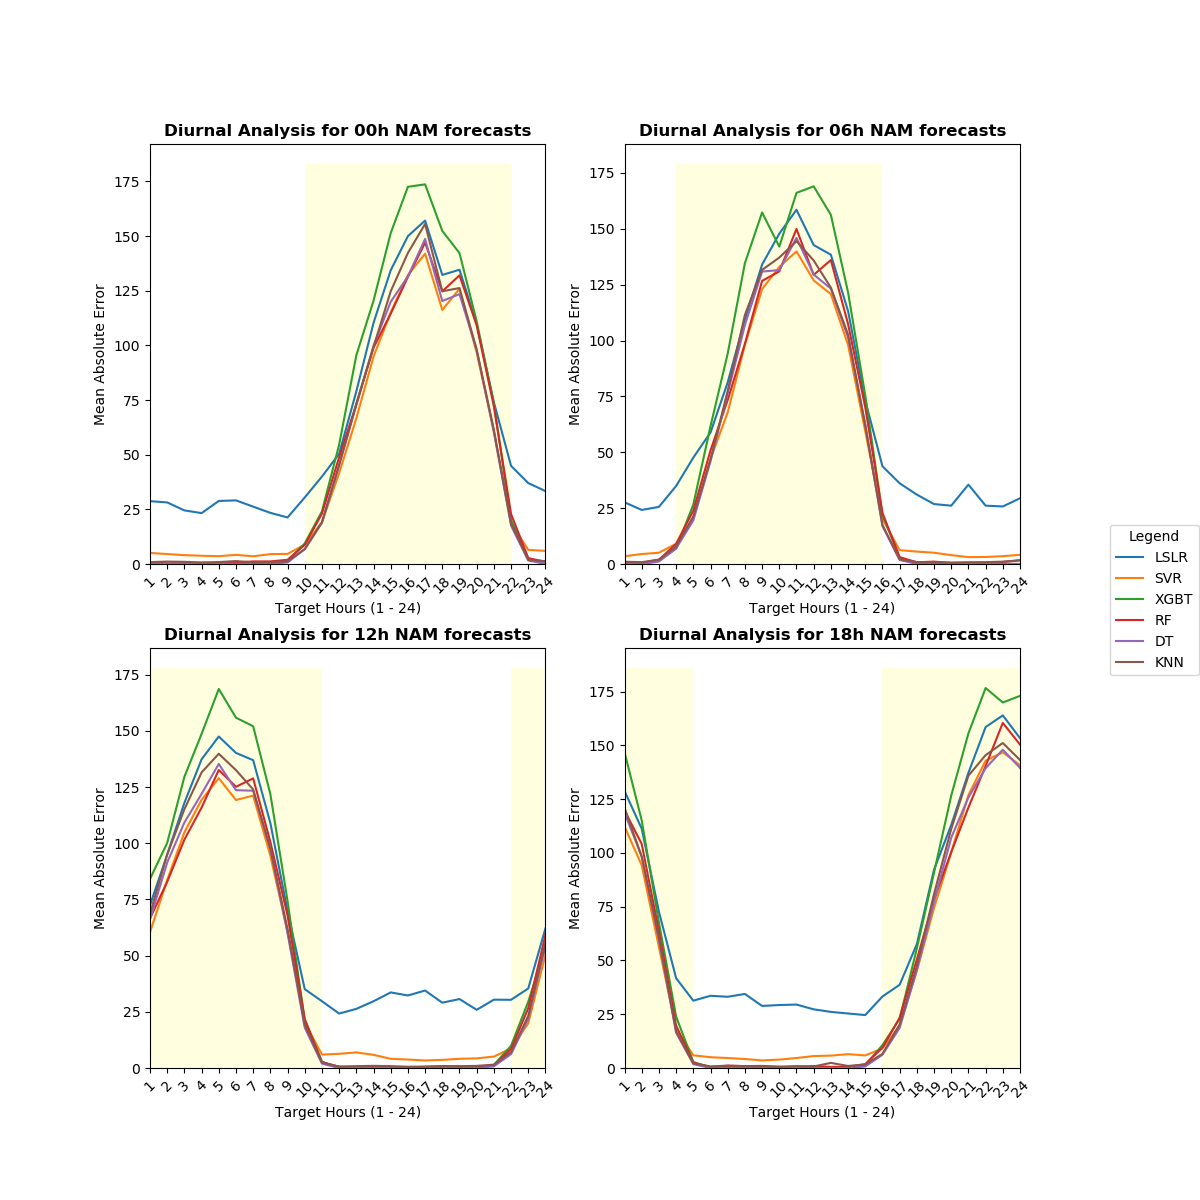
\includegraphics[width=0.9\textwidth, height=12cm]{chapter3/fig_diurnal_arrayb.png}
    	\caption[Stratified diurnal analysis of day-ahead irradiance predictions for fixed-axis solar array]{Stratified diurnal analysis of day-ahead irradiance predictions for fixed-axis array: (left-top) 00h NAM forecasts, (right-top) 16h NAM forecasts, (left-bottom) 12h NAM forecasts, (right-bottom) 18h NAM forecasts. Local time of day (6A.M to 6P.M) at the target location for each of the NAM forecasts is indicated in light yellow.}
    	\label{fig:fig_stratified_diurnal}
    \end{center}
\end{figure}

\par NAM forecasts are released at 00h, 06h, 12h and 18h UTC. In order to assess the performance of the machine learning models as a result of incorporating the input-selection scheme better, a stratified analysis was carried out. The mean absolute error (MAE) of the models for each of the target hours in the forecast horizon, i.e. between 1 and 24 was compared for all four types of NAM forecasts individually.

\par For using weather data from NAM Forecast System for training with the machine learning models, the reference times of the NAM forecasts were made time-zone aware with respect to the target location, i.e. Athens, Georgia. For the reference times corresponding to each of the NAM forecasts, corresponding solar irradiance observations were collected. The target location is -5.00 hours with respect to UTC in the standard time zone, and -4.00 hours with respect to UTC during \textit{daylight saving time}. For the sake of a diurnal analysis, it was assumed that the target location is -4.00 hours with respect to UTC throughout the year. 

\par Thus, 00h, 06h, 12h, 18h NAM forecasts each correspond to 8 P.M, 2 A.M, 8 A.M and 2 P.M locally. In Figure~\ref{fig:fig_stratified_diurnal}, for each of the NAM forecasts, local \textit{time of day} (i.e. between 6.00 AM and 6.00 PM) was identified. In the forecast horizon, i.e. in the consequent 24 hours, for each of the NAM forecasts, such \textit{time of day} was marked in yellow, so as to signify daytime. In Figure~\ref{fig:fig_stratified_diurnal}, it can be seen that the performance of most of the machine learning models is comparable regardless of day-time or night-time. While the \textit{support vector regression} models performed well during daytime, they performed slightly worse during night-time, only performing better than the simple \textit{linear regression}. The stratified diurnal analysis was essential in realizing that the performance of the models in Tables~\ref{Tab:fs_array_a}, \ref{Tab:fs_array_b} and \ref{Tab:fs_array_e} is misleading, as a much higher $MAE$ can be observed for certain target hours in the \textit{time of day}, for each of the forecasts.

\begin{figure}[ht]
    \begin{center}
    \subfloat[Local time analysis of NAM forecasts]{
    	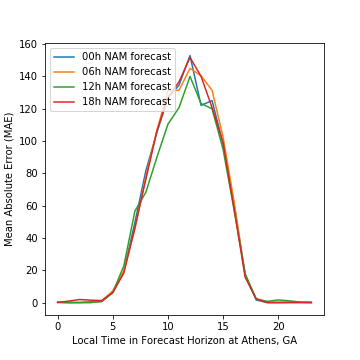
\includegraphics[width=0.5\textwidth, height=8cm]{chapter3/fig_time_shift_analysis.png}        }
%    \hspace{5mm}
    \subfloat[Model comparison at noon (local time)]{
    	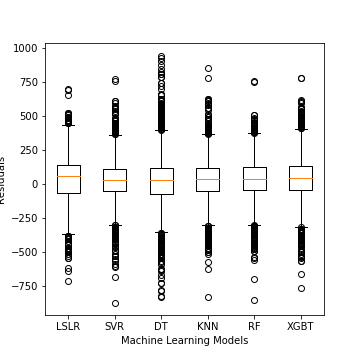
\includegraphics[width=0.5\textwidth, height=8cm]{chapter3/fig_noon_whisker.png}
        }
	\caption[Model performance comparison at different times in a day at the target location.]{ (a) Average performance of different target hours in the forecast horizon corresponding to each of 00h, 06h, 12h, 18h NAM forecasts, adjusted according to local time. 
	(b) Comparison of box-and-whisker plots of residuals from different predictive models utilizing GHI at 12 P.M local time, i.e. noon.}
	\label{fig:local_time_analysis}
    \end{center}
\end{figure}

\par In order to get a better understanding of the performance of the models, a local-time analysis was done. For each of the NAM forecasts, the forecast horizon corresponds to the following time ranges with respect to the target location: 9 P.M - 8 P.M, 3 A.M - 2 A.M, 9 A.M - 8 P.M, 3 P.M - 2 P.M. From these local time ranges, the predictions obtained from the \textit{random forests} algorithm corresponding to target hours representing the same local time were sampled together. $MAE$ was estimated for each of these groups, so as to attain the model performance at a certain time in a day, at the target location. In Fig.~\ref{fig:local_time_analysis}(a), this was plotted for each of the 00h, 06h, 12h, 18h NAM forecasts. The worst performance, expectedly, was observed at 12.00 P.M (local time) or noon. Such an analysis helps realize that for day-ahead solar forecasting with quality weather forecast data, the local time for which the prediction is being made is key to the quality of the prediction, than how farther away the target hour is in the forecast horizon.

\par In order to ascertain the better machine learning model at the local time most difficult to predict solar irradiance for, the quality of prediction of all machine learning models at 12 P.M (local time) was compared. To enable this, in Fig.~\ref{fig:local_time_analysis}(b), box-and-whisker plots were drawn for the residuals of the predictions from all the models at this time. It was observed that the \textit{random forests} had the least dispersion beyond the whiskers, indicating its effectiveness in irradiance prediction irrespective of the position of the target hour in the forecast horizon, or the local time of the target hour.

\newpage